\section{HW/SW Co-Design \weekDoran{1}}
	\subsection{System Architecture Specification}
	
		\begin{compactitem}
		  \item Specifies the individual components of a system.
		  \item Arrows indicate data flow
		  \item {\color{red}\textbf{THE BUS IS AN ACTIVE ELEMENT!!!}}
		  \item Elements that can compute things but are only used as passive components (like memory) are drawn as memories.
		\end{compactitem}
		
		\begin{multicols}{2}
			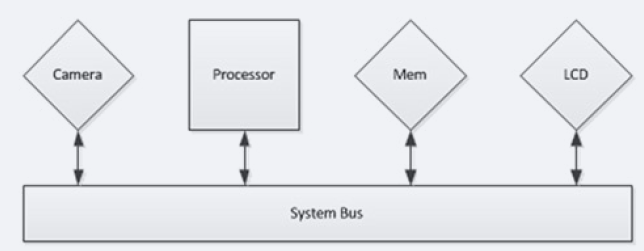
\includegraphics[width=0.4\textwidth]{./pictures/systemArchDiagram.png} \\
			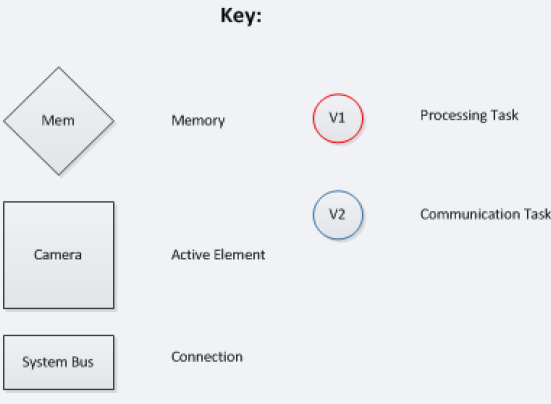
\includegraphics[width=0.4\textwidth]{./pictures/systemArchKey.png}
		\end{multicols}	

	\subsection{Bindings}
		\begin{multicols}{2}
			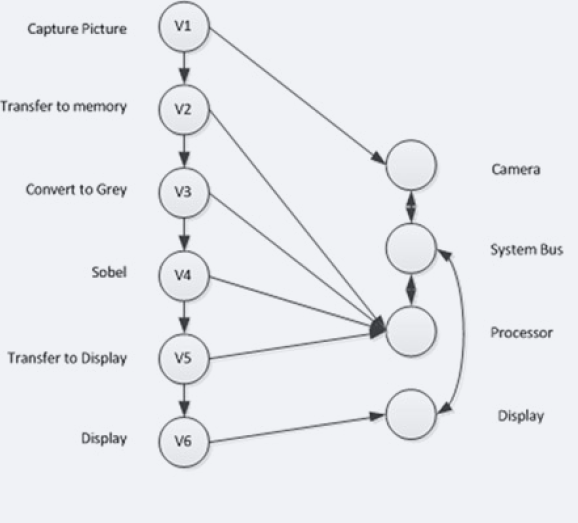
\includegraphics[width=0.4\textwidth]{./pictures/bindings.png} 
			\begin{compactitem}
			  \item The left part of the binding diagram shows the program flow, with each task as a bubble and arrows that indicate the flow. 
			  \item The right part of the binding diagram shows the system elements, with each element as a bubble. The arrows between the elements are the same data flow connections as in the system architecture diagrams.
			  \item The arrows between the left and the right side of the binding diagram indicate which elements are affected by which tasks.
			\end{compactitem}		
		\end{multicols}